\section{Theorie}
\label{sec:Theorie}

\subsection{Kathodenstrahlröhre}
\label{sec:Kathodenstrahlröhre}

Zur Erzeugung eines Elektronenstrahls wird eine Kathodenstrahlröhre, wie sie in Abbildung \ref{fig:rohr} zu sehen ist, verwendet.
\begin{figure}
  \centering
  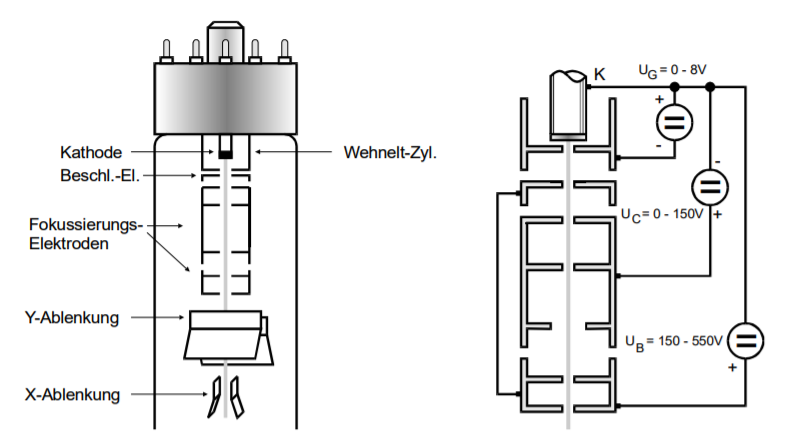
\includegraphics[height=7cm]{data/Kathodenstrahlrohr.png}
  \caption{Kathodenstrahlröhre.}
  \label{fig:rohr}
\end{figure}
Die Elektronen werden durch thermische Emission freigesetzt und durch eine Elektrode mit hohem positiven Potential beschleunigt.
Vor dem Ablenksystem, das aus einem horizontal und einem vertikal angeordnetem Plattenkondensator besteht, befinden sich Elektroden zur Fokusierung des Strahls.
Der Elektronenstrahl wird mit Hilfe eines Leuchtschirms registriert, dessen Atome durh die Elektronen zur Emission von Lichtquanten angeregt werden.
Außerdem herrscht im Inneren der Kathodenstrahlröhre ein Hochvakuum, um Wechselwirkungen der Elektronen mit Luftmolekülen zu verhindern.

\subsection{Ablenkung eines Elektronenstrahls im elektrischen Feld}
\label{sec:elekAblenkung}

Die Beziehung zwischen der Ablenkspannung $U_\text{d}$ und der Verschiebung des Leuchtflecks $D$ lässt anhand folgender Skizze \ref{fig:Ablenkung} herleiten.
\begin{figure}
  \centering
  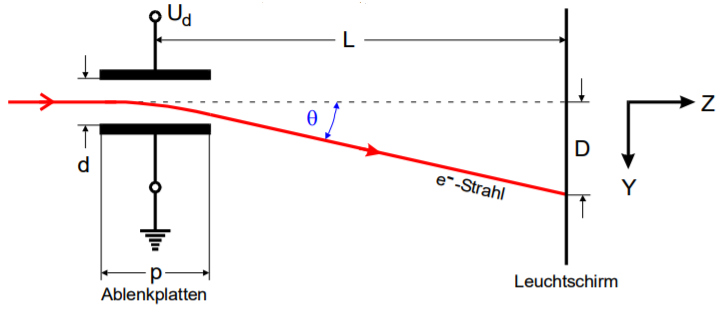
\includegraphics[height=7cm]{data/elekAblenkung.png}
  \caption{Ablenkung des Elektronenstrahls im elektischen Feld.}
  \label{fig:Ablenkung}
\end{figure}
$d$ bezeichnet dabei den Plattenabstand, $p$ die Plattenlänge, $L$ den Abstanden zwischen Ablenkplatten und Schirm und $\phi$ den Ablenkwinkel.
Zunächst müssen die Geschwindigkeitskomponenten in y- und z-Richtung bekannt sein, um die Ablenkung zu bestimmen.
Die z-Komponente lässt sich aus der kinetischen Energie eines Elektrons berechnen:
\begin{equation}
  v_z^2 = 2 \frac{e_0}{m_0} U_\text{B}
\end{equation}
Das Feld zwischen den Ablenkplatten kann als homogen betrachtet werden und so wirkt in x-Richtung die Kraft:
\begin{equation}
  F = e_0 \frac{U_\text{d}}{d}
\end{equation}
Das Elektron wird in der Zeit $\increment t = P / v_z$ auf folgende Geschwindigkeit beschleunigt:
\begin{align}
  v_y & = \frac{e_0}{m_0} \frac{U_\text{d}}{d} \increment t \\
  v_y & = \frac{e_0}{m_0} \frac{U_\text{d}}{d} \frac{p}{v_z}
\end{align}
Aus der Beziehung zwischen Ablenkwinkel $\phi$, $L$ und $D$ bzw. den Geschwindigkeitskomponenten lässt sich eine Gleichung für die Verschiebung aufstellen.
\begin{equation}
  D = \frac{p}{2d} L \frac{U_\text{d}}{U_\text{B}}
\end{equation}

\subsection{Kathodenstrahl-Oszillograph}
\label{sec:Oszillograph}

Die Kathodenstrahlröhre kann zu einem Oszillographen erweitert werden, indem an die horizontalen Ablenkplatten eine Sägezahnspannung und an die vertikalen Platten eine zu untersuchende Wechselspannung angelegt wird.
Bilden die Freqeunz der Sägezahnspannung $\nu_\text{Sä}$ und der Wechselspannung $\nu_\text{We}$ ein rationales Verhältnis, steht das Bild auf dem Leuchtschrim.

\subsection{Ablenkung eines Elektronenstrahls im magnetischen Feld}
\label{sec:magnAblenkung}

Im magnetischen Feld wirkt auf bewegte Ladung die Lorentzkraft, die für eine Ladung $q$ mit Geschwindigkeit $\vec{v}$ im homogenen Magnetfeld $\vec{B}$ wie folgt aussieht:
\begin{equation}
  \vec{F_\text{L}} = q \, \vec{v} \times \vec{B}
\end{equation}
Da in der Anordnung dieses Experimentes Geschwindigkeit, Magnetfeld und Kraft senkrecht aufeinander stehen, wird keine Arbeit an dem Teilchen verrichtet.
Also bleiben kinetische und potentielle Energie konstant und das Teilchen bewegt sich auf einer Kreisbahn.
Die Lorentzkraft fungiert dabei als Zentripetalkraft und so gilt für den Kreisradius:
\begin{equation}
  r = \frac{m_0 v}{e_0 B}
  \label{eqn:radius}
\end{equation}

\subsection{Bestimmung der spezifischen Elektronenladung}
\label{sec:Elektronenladung}

Die durch die Kreisbahn hervorgerufene Ablenkung kann nun dazu genutzt werden, die spezifische Elektronenladung zu bestimmen.
\begin{figure}
  \centering
  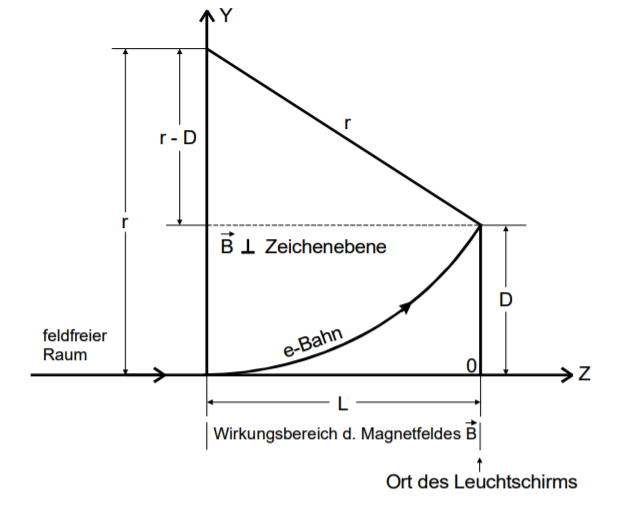
\includegraphics[height=7cm]{data/Kreisablenkung.png}
  \caption{Ablenkung auf Kreisbahn durch magnetisches Feld.}
  \label{fig:Kreis}
\end{figure}
Mit Gleichung \eqref{eqn:radius} und Abbildung \ref{fig:Kreis} lässt sich eine Beziehung aufstellen, die nur von Konstanten, der Geschwindigkeit $v_0$ und dem Magnetfeld $B$ abhängt:
\begin{equation}
  \frac{L^2 + D^2}{2D} = \frac{m_0 v_0}{e_0 B}
\end{equation}
Die Größen $v_0$ und $B$ können über die an die Kathodenstrahlröhre und an die Spulen angelegten Spannungen bestimmt werden.
